
%(BEGIN_QUESTION)
% Copyright 2012, Tony R. Kuphaldt, released under the Creative Commons Attribution License (v 1.0)
% This means you may do almost anything with this work of mine, so long as you give me proper credit

An engineer contacts you to help her troubleshoot a chemical problem in an ammonium nitrate process, where this compound is created by mixing ammonia vapors with nitric acid.

Analytical controller AIC-28 has been placed in manual mode for the purpose of maintaining a constant ratio of ammonia to nitric acid entering the neutralizer vessel.  AIC-28's output has been set at an ammonia:acid value that the plant's chemical engineer predicts should yield optimum results.  However, the chemical composition of the product exiting the neutralizer proves to be off spec, as though the ammonia to acid ratio is too lean (i.e. too little ammonia per unit measure of acid entering the vessel).  Flow ratio controller FFC-23's task is to maintain the proper flow ratio of ammonia to acid:

$$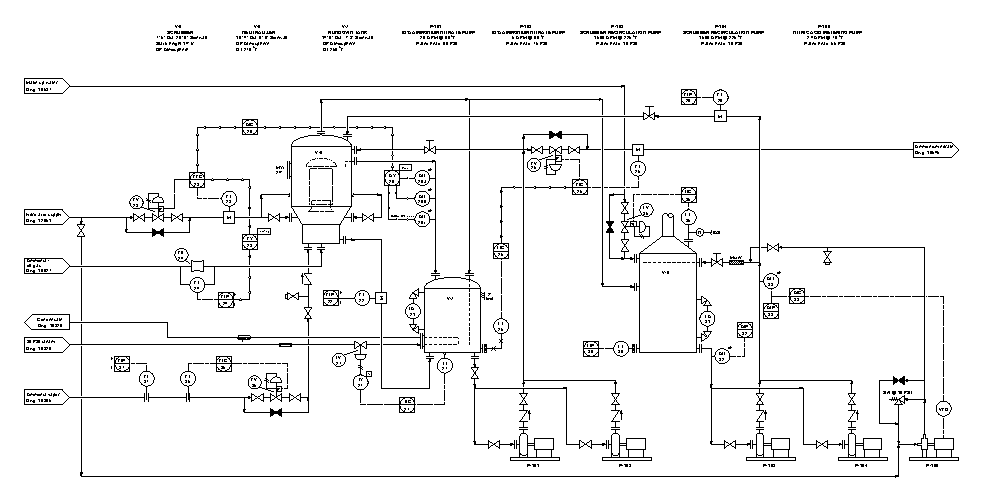
\includegraphics[width=15.5cm]{i0008rx01.eps}$$

Identify the likelihood of each specified fault in this process.  Consider each fault one at a time (i.e. no coincidental faults), determining whether or not each fault could independently account for {\it all} measurements and symptoms in this process.

% No blank lines allowed between lines of an \halign structure!
% I use comments (%) instead, so that TeX doesn't choke.

$$\vbox{\offinterlineskip
\halign{\strut
\vrule \quad\hfil # \ \hfil & 
\vrule \quad\hfil # \ \hfil & 
\vrule \quad\hfil # \ \hfil \vrule \cr
\noalign{\hrule}
%
% First row
{\bf Fault} & {\bf Possible} & {\bf Impossible} \cr
%
\noalign{\hrule}
%
% Another row
Bypass valve around FV-23 left open &  &  \cr
%
\noalign{\hrule}
%
% Another row
Plugged impulse line on FT-24 &  &  \cr
%
\noalign{\hrule}
%
% Another row
FT-23 calibration error (high) &  &  \cr
%
\noalign{\hrule}
%
% Another row
FT-23 calibration error (low) &  &  \cr
%
\noalign{\hrule}
%
% Another row
FT-24 calibration error (high) &  &  \cr
%
\noalign{\hrule}
%
% Another row
FT-24 calibration error (low) &  &  \cr
%
\noalign{\hrule}
%
% Another row
Nitric acid supply line plugged &  &  \cr
%
\noalign{\hrule}
%
% Another row
Ammonia off-gas line plugged &  &  \cr
%
\noalign{\hrule}
%
% Another row
Ammonia vapor line plugged &  &  \cr
%
\noalign{\hrule}
} % End of \halign 
}$$ % End of \vbox

Finally, identify the {\it next} diagnostic test or measurement you would make on this system.  Explain how the result(s) of this next test or measurement help further identify the location and/or nature of the fault.


\vskip 20pt \vbox{\hrule \hbox{\strut \vrule{} {\bf Suggestions for Socratic discussion} \vrule} \hrule}

\begin{itemize}
\item{} Identify each type of flowmeter shown in this diagram, based on the P\&ID symbols used.
\item{} Assuming FV-23 is air-to-open (fail-closed) identify the proper control action for FFC-23 (either direct or reverse).
\item{} Explain why this system uses three pH transmitters (AIT-28a, b, and c) rather than just one.
\item{} Explain what would happen in this system if FT-36 failed with a high signal.
\item{} Explain what would happen in this system if TT-27 failed with a high signal.
\item{} Explain what would happen in this system if LT-26 failed with a low signal.
\end{itemize}

\underbar{file i03501}
%(END_QUESTION)





%(BEGIN_ANSWER)


%(END_ANSWER)





%(BEGIN_NOTES)

Given the fact that we have too little ammonia (or too much acid), flow transmitter calibration errors are likely.  If FT-23 (acid flow transmitter) is reading lower than it should, this would cause the acid flow control loop to add too much acid.  If FT-24 (ammonia flow transmitter) is reading greater than it should, this would cause the acid control loop to put in too much acid (thinking more was needed than what is actually needed).

% No blank lines allowed between lines of an \halign structure!
% I use comments (%) instead, so that TeX doesn't choke.

$$\vbox{\offinterlineskip
\halign{\strut
\vrule \quad\hfil # \ \hfil & 
\vrule \quad\hfil # \ \hfil & 
\vrule \quad\hfil # \ \hfil \vrule \cr
\noalign{\hrule}
%
% First row
{\bf Fault} & {\bf Possible} & {\bf Impossible} \cr
%
\noalign{\hrule}
%
% Another row
Bypass valve around FV-23 left open & ? &  \cr
%
\noalign{\hrule}
%
% Another row
Plugged impulse line on FT-24 & $\surd$ &  \cr
%
\noalign{\hrule}
%
% Another row
FT-23 calibration error (high) &  & $\surd$ \cr
%
\noalign{\hrule}
%
% Another row
FT-23 calibration error (low) & $\surd$ &  \cr
%
\noalign{\hrule}
%
% Another row
FT-24 calibration error (high) & $\surd$ &  \cr
%
\noalign{\hrule}
%
% Another row
FT-24 calibration error (low) &  & $\surd$ \cr
%
\noalign{\hrule}
%
% Another row
Nitric acid supply line plugged &  & $\surd$ \cr
%
\noalign{\hrule}
%
% Another row
Ammonia off-gas line plugged &  & $\surd$ \cr
%
\noalign{\hrule}
%
% Another row
Ammonia vapor line plugged & $\surd$ &  \cr
%
\noalign{\hrule}
} % End of \halign 
}$$ % End of \vbox

The bypass valve being left open is only possible if the bypass valve's flow exceeds the desired acid flow even with FV-23 shut.  Otherwise, the ratio control system will still be able to maintain the correct ratio.








\vskip 20pt \vbox{\hrule \hbox{\strut \vrule{} {\bf Virtual Troubleshooting} \vrule} \hrule}

This question is a good candidate for a ``Virtual Troubleshooting'' exercise.  Presenting the diagram to students, you first imagine in your own mind a particular fault in the system.  Then, you present one or more symptoms of that fault (something noticeable by an operator or other user of the system).  Students then propose various diagnostic tests to perform on this system to identify the nature and location of the fault, as though they were technicians trying to troubleshoot the problem.  Your job is to tell them what the result(s) would be for each of the proposed diagnostic tests, documenting those results where all the students can see.

During and after the exercise, it is good to ask students follow-up questions such as:

\begin{itemize}
\item{} What does the result of the last diagnostic test tell you about the fault?
\item{} Suppose the results of the last diagnostic test were different.  What then would that result tell you about the fault?
\item{} Is the last diagnostic test the best one we could do?
\item{} What would be the ideal order of tests, to diagnose the problem in as few steps as possible?
\end{itemize}

%INDEX% Process: ammonium nitrate production (realistic P&ID shown)

%(END_NOTES)


